\newpage
\section{Product}
\label{sec:product}

Products are represented by ProductTypes.

\begin{figure}[ht]
	\centering
  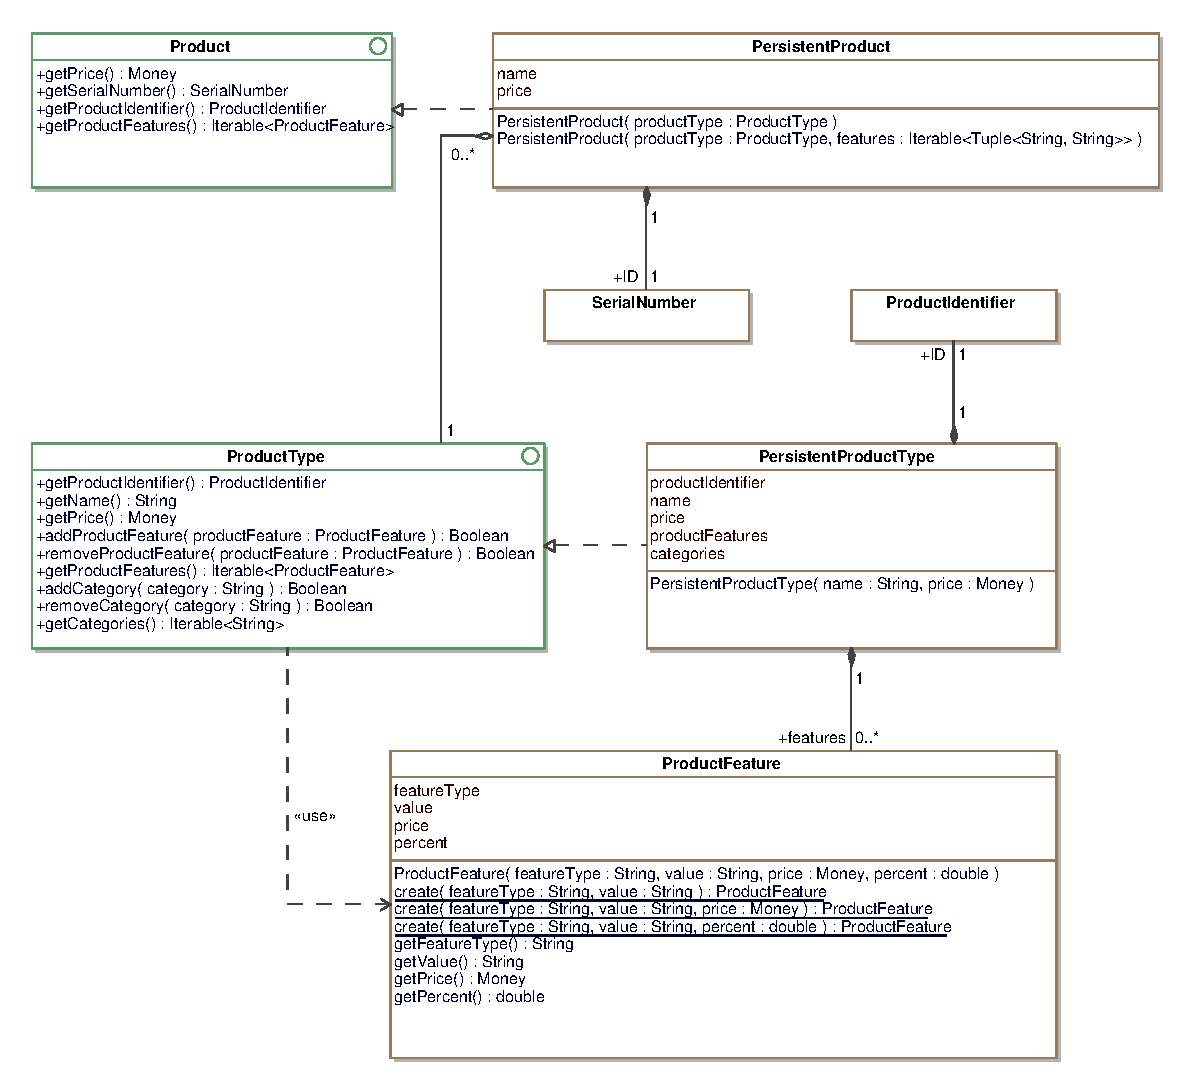
\includegraphics[width=1.0\textwidth]{images/Product_Overview.eps}
	\label{product_overview}
	\caption{Product - Class Overview}
\end{figure}

\subsection{\code{ProductType} - Representing specified products}
A \code{ProductType} is an interface which represents a specified product. The \code{PersistentProductType}-class is an implementation of this interface to worked with it.
An \code{PersistentProductType} contains \code{ProductFeatures} to specify your product. You can add any \code{ProductFeatures}  to this set or remove them from it.
An example: Our specified \code{ProductType} is a table. About to sell any variations of this table, you need any \code{ProductFeatures} like its color or the material of it. 
Also you can add categories to your \code{ProductType}, in this case you would choose the category: furniture or living room.

\subsection{\code{ProductFeature} - Creating Features}
Every \code{ProductFeature} has a featureType, a value and a price, which define it. Any {\code{ProductFeatures}} can offer the same featureType. For example the features red or green 
offer the featureType color. Mahogany, oak or beech offer the featureType wood.\\
The value defines the number of this \code{ProductFeature} in its \code{ProductType}. If you want to create a table, which offered four table-legs, then your table has a \code{ProductFeature} 
table-leg with value 4.   

\subsection{\code{Product} - Representing ProductTypes}
A \code{Product} is an interface which represents one specified \code{ProductType}. The \code{PersistentProduct}-class is an implementation of this interface to worked with it.
If you create a \code{PersistentProduct}, it gets a \code{SerialNumber} ,the \code{ProductIdentifier} of its \code{PersistentProductType} and the price will be calculated.
\code{SerialNumber} and \code{ProductIdentifier} are unique \code{SalespointIdentifier} to identify \code{ProductInstances} and \code{ProductTypes} in the database. 
There are subclasses of \code{ProductType} and \code{Product}, which extends the functionality of them. The subclasses of \code{ProductType} are \code{ServiceType} and 
\code{MeasuredProductType}, the subclasses of \code{Product} are \code{Service} and \code{MeasuredProduct}. 

%\subsection{\code{ServiceType} - Realizing Services}
%The interface \code{ServiceType} is implemented by the class \code{PersistentServiceType}. With this class you can realize services in your implementation, which represents a process 
%or activity that is offered for sale, for example a haircut on a barber shop or a driving lesson on a driving school.\\
%Every \code{PersistentServiceType} has a name and a price and can contains a start time and an end time. Between these dates the \code{PersistentServiceType} can be executed. If these dates 
%don't exist, the \code{PersistentServiceType} always is offered.

%\subsection{\code{Service} - Representing ServiceTypes}
%The interface \code{Service} is implemented by \code{PersistentService}, which represents one specified \code{PersistentServiceType}. The \code{PersistentService} has a 
%start time and an end time like its \code{PersistentServiceType}. The start time must be after the start time of \code{PersistentServiceType} and before the end time of 
%\code{PersistentService}. The end time must be before the end time of \code{PersistentServiceType}.\\
%Otherwise it will be thrown exceptions:
%\begin{itemize}
%\item \code{IllegalArgumentException}: If the \code{Service} end before it starts.
%\item \code{IllegalArgumentException}: If the \code{Service} begin before the period of \code{ServiceType} has begun.
%\item \code{IllegalArgumentException}: If the \code{ServiceType} end after the period of \code{ServiceType} was finished.
%\end{itemize}
%Also you can cancelled the \code{PersistentService} with the method \code{public void cancelServiceInstance()} and so the end time is now and you can get the 
%\code{ServiceDeliveryStatus} of the \code{PersistentService} at every time.
%  
%\subsection{\code{ServiceDeliveryStatus}}
%The \code{ServiceDeliverystatus} is an enumeration with follow attributes:
%\begin{itemize}
%\item \code{SCHEDULED}: If the start of the \code{Service} is in the future.
%\item \code{EXECUTING}: If the \code{Service} is executing now.
%\item \code{CANCELLED}: If the \code{Service} was cancelled.
%\item \code{COMPLETED}: If the \code{Service} is completed, so the end of the \code{Service} is in the past and it wasn't cancelled.
%\end{itemize}

\subsection{\code{MeasuredProductType} - Creating MeasuredProducts}
The interface \code{MeasuredProductType} is implemented by \code{PersistentMeasuredProductType}. If you use the functionality of this interface, you can realize products, which are not sold as 
predefined unit, but rather as measures of something. For example flooring may be sold by square foot or fresh products by kilogram.
A \code{PersistentMeasuredProductType} has a name, a price and a quantity on hand. The quantity on hand, is the quantity of this \code{PersistentMeasuredProductType}, which is available to 
be sold. You can also add or reduce a specified quantity of the \code{PersistentMeasuredProductType} to it. 
The price of the \code{PersistentMeasuredProductType} is not the price for an unit of that, but the price of the quantity on hand of that. The unit price will be calculated automatically 
and you can get it with the method \code{getUnitPrice()}.

\subsection{\code{MeasuredProduct} - Representing MeasuredProductTypes}
The interface \code{MeasuredProductType} is implemented by \code{PersistentMeasuredProductType}, who represents a specified quantity of the \code{PersistentMeasuredProductType}. After you 
create it, the quantity of that, will be reduce from the quantity on hand of the \code{PersistentMeasuredProductType}, because this quantity is used and no more available for other 
\code{PersistentMeasuredProducts}. If this quantity is greater than the quantity on hand, an exception will be thrown.
